%%\documentclass[CEJCS,DVI]{cej} % use DVI command to enable LaTeX driver
\documentclass[CEJCS,PDF]{cej} % use PDF command to enable PDFLaTeX driver
\usepackage{layout}
\usepackage{amsmath}
\usepackage{textcomp}
%\usepackage{algorithm}
\usepackage{algorithmic}
\algsetup{indent=.2in}
\usepackage{float}
\floatstyle{ruled}
\newfloat{algorithm}{thp}{lop}

\usepackage{moreverb}
\usepackage{graphicx}
\usepackage{caption}
\usepackage{url}
%% Place article title here:
\title{Scalable N-Body Event Prediction}
%% Place for inserting article category: Research Article, Review Article,
%% Communication or Vision Article
\articletype{Research Article}

\author{Steven Braeger\inst{1}\email{steve@soapforge.com},
        Nicholas Arnold\inst{1}\email{narnold@knights.ucf.edu},
        Damian Dechev\inst{1}\email{damian.dechev@gmail.com}}

\institute{
     \inst{1} University of Central Florida,\\
     4000 Central Florida Blvd., 32816 Orlando, Florida, USA
          }

%% Please type your abstract here.
\abstract{The general simulation of n-body systems often requires the simulation of pairwise interaction events between the objects.  The naive method of simulating these events is an algorithm that polls each pair of objects for an interaction every time-step.  This algorithm has $O(n^2)$ operations per time-step in the number of objects.  However, this method scales very well to multiple cores. In this paper, we propose a novel method of pairwise simulation that saves a significant amount of computation time by predicting possible future outcomes rather than reacting to them.  We demonstrate the implementation of this method, as well as demonstrate that it has amortized $O(n)$ complexity per time-step.  We also demonstrate an implementation to allow this algorithm to scale comparably well to multiple cores of a shared memory machine.}

%% Keywords should be separated by \*\ sign
\keywords{n-body systems |*| non-blocking synchronization |*| discrete event simulation |*| prediction}


\begin{document}
\maketitle

%% ###################################################################

\hyphenation{time-step}
\hyphenation{time-steps}

\section{Introduction}

There is a great deal of interest in discrete event simulation as it applies to video games and real time simulation. One interest in particular is the application of realistic physics in these simulations.  This kind of discrete event simulation is traditionally performed on large scale parallel clusters for film and scientific applications, or on massively parallel GPU architectures \cite{grape,uberflow}.  Specifically, we wish to explore the simulation and evolution of systems of dynamic and static objects where all the dynamic objects interact with all of the other objects, as happens when the dynamic objects physically collide with other objects.  In order to do this, we need to be able to model and react to collisions and interactions between objects. 

Although the naive and semi-naive implementations of this kind of simulation are embarrassingly parallel, they are also exceedingly wasteful.  The method used to evaluate the interactions between objects is similar to a busy-wait loop, where all objects are continually polled, waiting for collisions to occur as the simulation progresses \cite{nbodycollisions,Moore88collisiondetection}.   As we will describe in the next sections, we are interested in using a novel predictive model along with a novel scalable n-body event queue data structure to attempt to make a new kind of economical collision simulation system.  This system does not perform wasteful checks when checks are unlikely and maintains much of the parallelism of the naive solution.

\section{Problem Definition}

As input, we are given a description of static objects, dynamic objects, and the geometry defining their boundaries.  We are also given initial states like position, acceleration and velocity of the objects in the system, and a set of rules to update those objects.  As output, we wish to compute the exact state of each object in the system for each of the $n$ time-steps $t_0, t_1, t_2, \ldots, t_n$.

For each object $o$ in the system, a subroutine is defined \texttt{update($o$,$dt$)}, which computes the state of the object in the next time-step, given the object state in the current time-step and a time $dt$ between time-step.  For each pair of objects $o1$ and $o2$, an additional subroutine is defined \texttt{collide($o1$,$o2$)} which computes the state of both $o1$ and $o2$ in the next time-step, assuming that the objects have collided during the current time-step.

\subsection{Naive Algorithm}

The brute force all-pairs solution is the naive solution to this problem as it is commonly implemented in games. This technique is known as a 'detection' technique because it relies on the idea of detecting a collision when it occurs instead of predicting a collision.  

\begin{algorithm}
\caption{Naive Algorithm}
\begin{algorithmic}
\FOR{each time-step $ti$}
	\FOR{each dynamic object $do$}
		\STATE update($do,dt$)  \COMMENT{$dt$ is the constant time-step difference}
		\FOR{each object $o$}
			\IF{check($do, o$)}
				\STATE collide($do, o, dt$)
			\ENDIF
		\ENDFOR
	\ENDFOR
\ENDFOR
\end{algorithmic}
\end{algorithm}

This technique is embarrassingly parallel, allowing a thread per dynamic object or even a thread per pair with minimal overhead.  However, it is extremely
wasteful, because there are $O(n^2)$ checks being made every single time-step, even if the likelihood of a collision has changed little since the last time-step \cite{Seningood}.  

Each of these $O(n^2)$ checks per time-step is computationally cheap individually, but when the number of objects is very great the computational overhead of performing all of them becomes
unmanageable. Considering that an extreme majority of the checks will fail due to the fact that collision occurrences are rare, most of them do not need to be computed, and avoiding their computation has the ability to dramatically increase the 
throughput of our simulation.

\subsection{Semi-Naive Algorithm}

A similar algorithm that we refer to as the 'semi-naive' algorithm has also found great use in practical applications \cite{Bittner02hierarchicaltechniques}.  The semi-naive algorithm differs is the same as the naive algorithm, except that it exploits a bounding volume hierarchy to spatially partition the dynamic objects and pre-filter the collision checks.  This algorithm is also wasteful in that most of its checks fail, but only has $O(n log n)$ checks if the objects are relatively equally distributed throughout the bounding space.

\section{Theoretical Contribution}
\label{sec:theocont}
\subsection{Predictive Algorithm}

In our desired solution, we take a completely different approach.  In contrast to the naive and semi-naive algorithms, our solution avoids computing any unneeded checks on time-steps that do not change the solution by \textit{predicting} the intersections before they occur, rather than checking for them when they do not.  Our algorithm will use a slightly more complex subroutine \texttt{predict($o1$,$o2$)} that returns the time an intersection is likely to occur, and enters it into an event queue that contains the predicted collisions that are likely to occur.  When an intersection occurs, it is recomputed and removed from the queue.

\begin{algorithm}
\caption{Predictive Algorithm}
\begin{algorithmic}
\STATE \COMMENT{initialize events from initial states} % future_event_queue()
\FOR{each time-step $ti$}
	\FOR{each dynamic object $do$}
		\STATE update($do,dt$)  \COMMENT{$dt$ is the constant time-step difference}
	\ENDFOR
	\STATE \COMMENT{for each event that occurs in this time-step}
	\FOR{each e in events.find(ti)}
		\FOR{each object $o$}
			\IF{check($e.o,o$)}
				\STATE collide($e.o, o, dt$) \COMMENT{predict next collision event into queue}
			\ENDIF
		\ENDFOR
		\STATE{$events$.remove($e$)}
	\ENDFOR
\ENDFOR
\RETURN events
\end{algorithmic}
\end{algorithm}

It is worth noting that although our solution has the same runtime complexity as the naive solution in the worst case (and, in fact, the initial population of event queue will need to perform $O(n^2)$ predictions), it is unlikely to compute ANY checks that are unlikely to occur, thus saving tremendous computation time in the average case.  

However, our work is not done.  This algorithm is difficult to parallelize when compared to the naive algorithm, as it depends implicitly on reading and writing the global future n-body event queue data structure described in section \ref{sec:neq}.  This data structure is a specialized queue in which events take priority over other events about to take place. If we split the evaluation of the simulation into threads, then each thread must somehow synchronize which events it will prioritize and avoid collisions.  Furthermore, threads must be able to communicate and respond to future events  globally as collisions are predicted into the future.  This communication overhead is difficult to parallelize correctly, and will be the focus of our research.

\subsection{N-Body Future Event Queue}
\label{sec:neq}
Our algorithm depends on a data structure we call an "N-Body Future Event Queue".  This data structure is designed to facilitate the prediction algorithm
by storing pairwise events that are probabilistically likely (but not guaranteed) to occur.  Such a data structure has the following pseudo-code description

\floatname{algorithm}{Data Structure}
\begin{algorithm}
\caption{Future Event Queue} % TODO: This didn't have a caption, so I input it
\begin{algorithmic}
\STATE \COMMENT{inserts an event into the queue, possibly superseding any events that happen later}
\STATE \textbf{insert}($event$)
\STATE \COMMENT{removes an event from the queue}
\STATE \textbf{remove}($event$)
	
\STATE \COMMENT{returns an iterator that iterates over all predicted events that occur after time $t$}
\STATE EventIterator \textbf{find}(time $t$)

\STATE \COMMENT{Returns all objects for which nothing is known about their behavior}
\STATE ObjectIterator \textbf{find\_invalid}()
\end{algorithmic}
\end{algorithm}

It is important to take special note here of the operations in the future event queue.  The most important differences from it and a standard priority queue or event queue
is that the find() method can search for all events that occur within a certain time-frame, and that events that get input into the queue are not necessarily persistent, as they 
may be superseded by events that are inserted later but are queued to occur before.  An event A in the queue supersedes an event B iff event A and B have an object in common AND A is scheduled to occur BEFORE B.

Lastly, ``find invalid'' is important because it is assumed that at some point some event will occur for each object. (If that was not true for a particular object o, then simulating o is 
useless).  Thus, any objects which are in the scene but not present in the future event queue would indicate an error in our simulation logic.  In our example, even objects which
will not collide with any other objects must eventually collide with the boundaries of the simulation volume.  If no such collisions were known about
an object, we must know of this immediately and attempt to re-predict that object's future.

In addition, our queue must implement these algorithms efficiently in order to preserve the desired average-case $O(n)$ that our prediction algorithm facilitates.  In particular, all operations must be implemented in $O(n)$ time.

\section{Scalable Implementation}
In this section, we propose a scalable implementation of the predictive algorithm from section \ref{sec:theocont}, including an implementation of the 
N-Body Future Event Queue data structure.  Our implementation uses barriers and hardware atomic compare-and-swap primitives to guarantee thread-safety.  Our scalable implementation
works in two parts, which we will discuss here:  First, it uses barriers and an hardware compare-and-exchange boolean to synchronize the algorithm that utilizes the data structure, 
a process that is described in Section \ref{sec:stsp}.  Next, it uses an array with a thread-safe indexing scheme to implement the future event queue which is described in Section \ref{feq}
\subsection{Barriers}
\label{sec:barrier}
A barrier is a construct that is crucial to any threaded simulation.  It is a simple synchronization primitive that only has one operation: wait(n).  
A thread that enters wait(n) will wait at that point in the control flow of the program until the total number of threads in the wait(n) function is n.  Then,
all threads return simultaneously.

Typically, a barrier is not classified as a lock-free operation.  In most implementations of a barrier, a locked mutex is used to sleep all the threads, which is 
unlocked when the number of sleeping threads is equal to n.  However, this need not be the case.  We observe that the barrier preserves the lock-free property if it is implemented
using a hardware atomic instruction instead.  Wait() can be implemented as the following pseudcode.

\floatname{algorithm}{Procedure}
\begin{algorithm}
\label{barrier}
\caption{Wait}
\begin{algorithmic}
\STATE barrier
	\STATE int $num\_threads$ \COMMENT{the number of threads to collect}
	\STATE wait()
	\STATE \COMMENT{collect this thread}
	\STATE fetch\_and\_sub($\&num\_threads$,1)
	\STATE \COMMENT{spin until all threads are collected}
	\WHILE {$num\_threads > 0$}
		\STATE noop()
	\ENDWHILE
	\STATE \COMMENT{uncollect this thread}
	\STATE fetch\_and\_add($\&num\_threads$, 1)
\end{algorithmic}
\end{algorithm}

When implemented in this way, the implementation preserves the lock-free property, because even though n-1 threads are forced to wait, the last thread never waits for any 
mutex, or does it ever enter the spin-lock loop.  The last thread does useful work until it enters the wait() body, then immediately exits, continuing to make progress, releasing all
other threads in the process.

\subsection{Scalable Timestep Sub-Phases}
\label{sec:stsp}
In all threaded implementations of time-step-based simulation, at least one barrier construct
is necessary in order to prevent the system from processing more than one time-step at a time.  Without an implicit barrier at the beginning or end of the 
processing for each time-step, then worker threads could easily get out of sync on the time-steps that they are working on, which would produce incorrect calculations
for comparisons between threads.  The current time-step of the simulation must be constant across all threads, and so a barrier is used in order to synchronize that time-step.  This
limitation is true for all threaded time-step simulation, our application included.

Therefore, we can consider the timespan of a single time-step as a single computational unit, the beginning and end of which all threads are operating in sync.  We can ignore
all processing that occurs outside of a single time-step.  For our implementation of the prediction algorithm described in \ref{sec:theocont}, a single time-step is broken down
into several distinct 'phases,` with the overall structure as follows:

\floatname{algorithm}{Procedure}
\begin{algorithm}
\caption{Timestep}
\begin{algorithmic}
\STATE check\_react\_collisions();
\STATE repredict();
\STATE update\_simulation();
\STATE time-step\_sync\_barrier.wait();
\end{algorithmic}
\end{algorithm}

Note the implicit barrier protecting all threads from moving to the next frame before their peers.  The implementation of each subroutine are given in section \ref{sec:subphase}.

The primary problem with thread safety in this formulation of the time-step is the program errors that can occur in the status of the queue and the determinism of the simulation
if multiple threads are in different phases simultaneously.  For example, if thread A is updating object j, in the ``update simulation stage'', and thread B is writing to object 
j and i in the ``check react collisions'' phase, then the exact results the simulation will calculate are non-deterministic based on processor scheduling.  
Due to the fact that there are 3 phases, and $n$ objects, the total number of possible non-deterministic phase-overlap outcomes is $3\times3\times n=9n$.  This is clearly not an thread-safe solution.

However, as can be seen from section \ref{sec:subphase}, each of the sub-phases can be parallelized somewhat trivially.  Additionally, each sub-phase either reads and writes
a single array for that phase without inter-thread communication, or reads and writes two arrays with inter-thread communication.  Therefore, to allow us to parallelize each
phase in isolation, we break up the time-step into ``sub-phases'' using an additional barrier operation, implemented as in section \ref{sec:barrier}.  

\floatname{algorithm}{Procedure}
\begin{algorithm}
\caption{Check\_React\_Collisions}
\begin{algorithmic}
\STATE \COMMENT{search event queue for events that are occurring now}
\FOR{$e$ in $events$.find($current\_time$)}
	\STATE \COMMENT{if the event happens}
	\IF{check($e.o1,e.o2$)}
		\STATE \COMMENT{modify both objects}
		\STATE collide($e.o1,e.o2$)
	\ENDIF
	\STATE \COMMENT{the event is passed, so remove it.}
	\STATE $events$.remove($e$)
\ENDFOR
\end{algorithmic}
\end{algorithm}

This way, we can guarantee that each thread never has cross-phase non-determinism, reducing the number of potential non-deterministic concurrency cases to account for from $9n$ to $3n$
Furthermore, as we will demonstrate, the update phase and the re-predict phase are embarrassingly parallel and require no cross-thread communication or synchronization,
reducing the synchronization concerns to only the implementation of check-react.

\subsection{Scalable Sub-phases}
\label{sec:subphase}

\subsubsection{Update}
\label{sub:update}
The update phase is simple and embarrassingly parallel.  It also demonstrates our overall technique to distribute work equally to multiple threads.  In most of our sub-phases,
we evenly distribute one object to perform operations on each thread, evenly, one at a time by using a hash function that maps object ids to thread ids evenly. $thread(object\_id) = object\_id \% num\_threads + thread\_id$
\floatname{algorithm}{Procedure}
%\begin{algorithm}
%\caption{Update\_Simulation}
\begin{algorithmic}
\FOR {every object $o$ assigned to $current\_thread$}
	\STATE update($o$)
\ENDFOR
\end{algorithmic}
%\end{algorithm}

Because updating an object only modifies that particular object, this phase is embarrassingly data-parallel and needs no additional synchronization.

Based on our definition of the problem and our use cases, we assume that the update() procedure has no explicit dependance on any of the other objects
in the system, only on some state internal to the object that allows us to move the simulation forward, such as internal velocity and position, and us $O(1)$.  This means
that the entire Update\_Simulation procedure is $O(n)$.
\subsubsection{Check-React}
\label{sub:checkreact}
\floatname{algorithm}{Procedure}
\begin{algorithm}
\caption{Check\_React\_Collisions}
\begin{algorithmic}
\STATE \COMMENT{search event queue for events that are occurring now}
\FOR{$e$ in $events$.find($current\_time$)}
	\STATE \COMMENT{if the event happens and this thread is assigned to it}
	\IF{$e$.$o1$ is in $current\_thread$ and check($e.o1,e.o2$)}
		\STATE \COMMENT{modify both objects}
		\STATE collide($e.o1,e.o2$)
	\ENDIF
	\STATE \COMMENT{the event is passed, so remove it.}
	\STATE $events$.remove($e$)
\ENDFOR
\end{algorithmic}
\end{algorithm}
This phase does the grunt work of the predictive algorithm.  During this phase, pending events that were predicted to happen in the current time-step are checked to see if they actually occur.  This phase requires additional synchronization overhead for several reasons.

\begin{enumerate}
	\item collide() reads and writes TWO objects, which means it could potentially modify objects that are assigned to other threads non-deterministically.
	\item There could be two events in the queue which actually describe the same event but swap the order of the objects, which could mean that a collide() reaction to the event could be triggered twice in the same frame.
	\item Multiple threads could check() an object while another object is in the middle of writing to it.
\end{enumerate}

However, we can exploit the structure of our problem in order to guarantee that none of these cases occur.  Due to the fact that for two symmetric events, we only want one... we can check to see if one or both of the objects in the set have already collided.
We can do this by using a flag bit for each of the objects in the scene to check whether or not the objects have collided yet this frame.  Then, we check
that bit for the OTHER object in our comparison, to see if the collision has already occurred.  Regardless of whether or not the bit is set, we wish to atomically
update the status of that bit to true for our current object.  The code becomes as follows.

\floatname{algorithm}{Procedure}
\begin{algorithm}
\caption{Check\_React\_Collisions}
\begin{algorithmic}
\STATE \COMMENT{search event queue for events that are occurring now}
\FOR{$e$ in $events$.find($current\_time$)}
	\STATE \COMMENT{if object reacted yet is false,set reacted to true and do the event}
	\IF{!compare\_and\_exchange(reacted\_yet[$e.o1$],false,true)}
		\STATE \COMMENT{if the event hasn't happened and this thread is assigned to it}
		\IF{$e.o1$ is in current\_thread and check($e.o1,e.o2$)}
			\STATE \COMMENT{modify both objects}
			\STATE collide($e.o1,e.o2$)
		\ENDIF
		\STATE \COMMENT{the event is passed, so remove it.}
		\STATE $events$.remove($e$)
	\ENDIF
\ENDFOR
\end{algorithmic}
\end{algorithm}

The complexity analysis of this procedure is non-trivial.  During Check\_React\_Collisions, the code in the loop is executed only if there is 
some collision that is predicted to occur during this time-step.  However, whether or not any collisions occur depends on a number of factors that
cannot be effectively reasoned about mathematically. For the purposes of our analysis in the rest of the section, let $k$ refer to the number 
of collisions that occur during the current time-step.  

To analyize this section, we make the reasonable assumption that collide(),check() and compare\_and\_exchange all have $O(1)$ complexity, so the complexity
of the loop is $O(k R(n))$, where $R$ is the complexity of $events$.remove(), which we will discuss later.  In addition, we must consider the complexity $F$
of the events.find() method in the overall procedure, which we will also discuss later.  Therefore the final complexity of this procedure is $O(F(n)+k R(n))$, which
becomes $O(F(n)+n R(n))$ in the worst case.

\subsubsection{Re-predict}
\label{sec:repredict}
The re-prediction phase is slightly more complex, but it is also embarrassingly parallel and scalable, provided that the implementation of our future event queue is thread-safe and scalable as well.  It detects simulation errors of the sort described in section \ref{sec:neq}, and also re-predicts collisions
that have been removed in check-react.  After finding all of the invalid objects (objects with no known future) that have been recently invalidated by check-react as well as logic errors, it then
searches for all known predictions that will occur in the future and puts them into the queue.  

\begin{algorithm}
\caption{Re-predict()}
\begin{algorithmic}
\STATE \COMMENT{search event queue for objects that the queue is unaware of}
\FOR{$oinvalid$ in $events$.find\_invalid($current\_time$)}
	\STATE \COMMENT{if invalid object is assigned to this thread}
        \IF{$oinvalid$ in current\_thread}
		\FORALL{dynamic\_objects $do$}
			\STATE $events$.insert(predict($oinvalid,do$))
		\ENDFOR
	\ENDIF
\ENDFOR
\end{algorithmic}
\end{algorithm}
This algorithm is thread-safe and scalable provided that the implementations of events.insert and events.find\_invalid are thread-safe and scalable, because predict is a read-only method that 
does not write to non-thread assigned data, even though it reads the current state of all dynamic objects in the scene.

The complexity of this procedure also depends on an unknown factor, which is the number of invalid entries in the queue, which we will call $k'$.  In most cases, $k=k'$, because objects are made invalid
when removed from the queue in the check-react phase.
The complexity of this procedure also depends on the complexity of the events.insert() procedure, which we label as $I(n)$.  We assume that predict() can be performed in constant time.
Therefore, this procedure runs in $O(F_i(n)+k' n I(n))$ time, where $F_i(n)$ is the complexity of find\_invalid() as defined in section \ref{feq}.

In the case of an empty future queue, this phase is $O(n^2 I(n))$, because it has to make predictions on all pairs of objects.  However, in order for that to occur in the average case would require a majority of frames to have all objects collide
with some other object simultaneously, a case which is exceedingly rare for the simulations we wish to run.

\subsection{Future Event Queue}
\label{feq}
The future event queue stores N-body events, and is designed to be used in concert with the sub-phase algorithm as described in Section \ref{sec:subphase}.
Our implementation uses an array to store a series of one-element priority-queues: one for each object in the scene.  This array shows the current best-guess
prediction of events that are inbound on the object.  The advantage of this approach is that our predictive queue doesn't have to deal with the contention of 
a standard queue implemented in a list, and it is also space efficient, as it is able to throw away events that supersede other events at insertion time.


\subsubsection{insert}

The implementation of insert is protected by the fact that an event that is inserted containing object $i$ as the first object in the event will only
be inserted from the thread that owns object $i$, as can be seen from section \ref{sec:repredict}.  Thus, insert requires no synchronization, as it can be verified
that no other thread will read or write to this same location during the react sub-phase.  

It is important to note that this implementation can and does remove events before they are checked from the queue,
and would not be suitable for any other kind of event queue.  However, our application domain says that removing potential events that will not occur from the queue is a feature, not a bug.
The repredict phase and the check-react phase work together to ensure the correctness of the algorithm despite the fact that these events can be removed.
For example, a pair of objects O1 and O2 may predict a collision may occur at time-step 60 in the future.  However, an object O3 may predict a collision with O1 at time-step 30.
This collision may NOT occur due to the fact that something else might occur between now and time-step 30, but it is still entered into the queue.  Thus, the check-react phase must double-check
all collisions in the queue for validity before reacting.  However, upon reaction to a collision that event is marked as invalid in the queue.  All invalid
objects are then recomputed.  In our example, the collision predicted at time-step 30 removes the collision predicted at time-step 60.  However,
if the first collision fails to occur, then during the repredict phase of time-step 30, the collision between O1 and O2 at time-step 60 would be re-discovered.

\begin{algorithm}
\caption{Insert}
\begin{algorithmic}
\STATE FutureEventQueue::insert(event $e$)
\IF{NOT(this.current\_events[$e.o1$].valid) or  $e$.time $<$ this.current\_events.time}
	\STATE this.current\_events[$e.o1$] = $e$;
\ENDIF
\end{algorithmic}
\end{algorithm}

This definition of insert runs in $O(1)$ time, as it only needs to access a particular element of the internal event array.  Therefore, $I(n)=O(1)$.

\subsubsection{remove}

Remove is similar to insert, except it simply sets the event to invalid in the array queue.

\begin{algorithm}
\caption{Remove}
\begin{algorithmic}
\STATE FutureEventQueue::remove(event $e$)
\STATE this.current\_events[$e.o1$].invalid;
\end{algorithmic}
\end{algorithm}

It runs in $O(1)$ time, for the same reason as ``insert()'', so $R(n)=O(1)$.

\subsubsection{find\_invalid}

The implementation of find\_invalid with our array-based queue is simply a linear search for any events that are marked as invalid in the array.
However, because of our previous rule that the event array cannot be read or written by a thread not its owner in the same phase, we only return invalid
objects from the objects in the current thread.  Although this would seem to break the functionality of find\_invalid, this behavior simply serves to reinforce
the constraint given in \ref{sec:repredict} that threads can only re-predict objects they own. It also means that we never re-predict objects across thread
ownership boundaries.  

\begin{algorithm}
\caption{Find\_Invalid}
\begin{algorithmic}
\STATE ObjectIterator FutureEventQueue::find\_invalid()
\FOR{o in dynamic\_objects}
	\IF{o in current\_thread AND !this.current\_events[o].valid }
		\STATE \COMMENT{return object as part of invalid set for this thread.}
		\STATE yield o;
	\ENDIF
\ENDFOR
\end{algorithmic}
\end{algorithm}

As it is implemented as a linear search through the array, Find\_invalid() is in $O(n)$.  


\subsubsection{find}

Similar to the implementation of find\_invalid, the implementation of find also is implemented based on a linear search.  It finds all valid events
and also checks to make sure that those events are happening in the current frame.

\begin{algorithm}
\caption{Find}
\begin{algorithmic}
\STATE EventIterator FutureEventQueue::find(current\_time)
\FOR{o in dynamic\_objects}
	\IF{o in current\_thread AND this.current\_events[o].valid AND this.current\_events[o].time <= current\_time}
		\STATE \COMMENT{ the event that is about to occur}
		\STATE yield this.current\_events[o];
	\ENDIF
\ENDFOR
\end{algorithmic}
\end{algorithm}

As it is also implemented as a linear search through the array, find() is in $O(n)$.

\subsection{Summary of Predictive Method}
	The sub-phase barriers and the thread object ownership system work together to ensure the thread-safety of the inputs and outputs to the Future Event Queue.
This partnership ensures in all the covered cases that the same object data is never used as a concurrent shared resource for both reading and writing.  In addition, we believe our algorithm maintains
the lock-free property because it remains wait-free in all states except when a thread is waiting at a barrier, which we justified is still a lock-free state in Section \ref{sec:barrier}.

\subsubsection{Complexity}

By examining the results from each of these analysis, we can analyze the complexity of the overall time-step in by looking at the total complexity for each of the sub-phases described in Section \ref{sec:stsp}.
From Section \ref{sub:checkreact} we see that the complexity of the check-react subphase is $O(F(n)+k R(n))$, which becomes $O(O(1)+kO(1))=O(k)$ after substuting our definitions of $F$ and $R$ from Section \ref{feq}.
From Section \ref{sub:update} the complexity of the update subphase is $O(n)$.  
Lastly, the complexity of the repredict subphase \ref{sec:repredict} is $O(F_i(n)+k' n I(n))$, which also reduces after substitution to $O(O(1)+k' n O(1))=O(k'n)$.

Because the final complexity per time-step is the complexity of all of the phases, the final time-step complexity is $O(k+n+k'n)$.  In the worst case $k'=k=n$, which occurs once during the initialization phase, and could occur with 
very low probability at any other time, then this reduces to $O(n^2)$.  However, experimentally and rationally, $k << n$, because the number of collisions
that are predicted to occur in any single timetep are guaranteed by the physical nature of our problem to be much less then $n$.  As a matter of fact, as seen in Section \ref{results}, in our experiments
$k=0$ in 90-98\% of the time-steps simulated.

\section{Experimental Setup}%Nick

In order to test our algorithm, we implemented a particular instance of future event simulation in the detection of collisions between two objects.

In typical instances of this problem in the real world, the type of simulation varies dramatically. In many applications, the objects obey complex interaction patterns such as flocking behavior and user interaction.  However, these interactions are almost always built around a simple framework for simulation that obeys Newtonian physics as the primary motion characteristic, with the more complex
behaviors simply activating different Newtonian trajectories and velocities \cite{Jadbabaie02coordinationof}.  Therefore, without loss of generality, we will simplify our simulation by limiting the object behaviors to simulate Newtonian physical interactions of objects under Earth-like gravity.

For our simulation, since we are using dynamic spheres, we use the following calculations for the collision reaction\cite{wheatchex}:

\begin{math}
c = n \cdot (v_{1i} - v_{2i})
\end{math}

\begin{math}
v_{1f} = v_{1i} - \frac{m_2 \cdot c}{m_1 + m_2} \cdot (1 + e)n
\end{math}

\begin{math}
v_{2f} = v_{2i} + \frac{m_1 \cdot c}{m_1 + m_2} \cdot (1 + e)n
\end{math}

where:

$v_{1i}$ = the initial velocity of object 1

$v_{2i}$ = the initial velocity of object 2

$m_1$ = the mass of object 1

$m_2$ = the mass of object 2

$e$ = the coefficient of restitution ($e$ = 1 for completely elastic)

$n$ = normal unit vector drawn from object 1 to object 2


Real simulations may also involve extremely complicated geometry, such as the convex shapes of human faces, vehicles, and buildings.  However, 
all of these simulations generalize objects by a first pass of a 'bounding volume' for the more complex object.  The bounding volume is a simple shape (e.g., a sphere)
that forms tight bounds on the object.  Real applications solve the first-pass collision checks for the simple 'bounding volume', and only fall back to a more complex
collision check on convex shapes if the bounding volumes intersect.  Thus, we can solve the problem without loss of generality by solving the problem
for simple bounding-volume shapes \cite{uberflow,cloth}.  In our case, we choose to use dynamic objects made of simple spheres, and static objects made of planes.

In order to program the simulation, we will use the latest version of the C++ standard, as it is a good language for high performance simulation applications.  In order to facilitate our 
3D geometry and numerical libraries, we will write our own simulation system and geometry routines based on the C++ Numerical Vector library Eigen \cite{eigenweb}.  

We wish to test performance economy as well as parallizability.  For our parallelization tests, we used thread-level parallelism and atomic primitives from the latest version of the C++ standard.

The performance of these systems is typically evaluated in terms of a throughput measurement that measures the number of time-steps per second the system is capable of evaluating.  Equivalently, one can measure the average wall-clock time that passes while evaluating one time-step.

\subsection{Naive Implementation}

The implementation of the naive solution is relatively straightforward, as a naive approach should be.  First, all of the dynamic objects must be updated for each time-step to their new positions, using their previously calculated velocity vectors.  Then, because we are handling the spheres and planes separately, we have two sets of nested for loops to perform the collision checks.  The first loops over the spheres and checks each with all of the planes, and the second loops over the spheres and checks each with all of the spheres that are after it in the list.  We do this to avoid checking each pair twice (\texttt{collide($o1$,$o2$)} would evaluate the same as \texttt{collide($o2$,$o1$)}). For the threaded version of this algorithm, we simply run outermost for loop in parallel:

\floatname{algorithm}{Algorithm}
\begin{algorithm}
\caption{Update}
\begin{algorithmic}
\FOR {$i = 0$ to $num\_spheres$}
	\STATE $dynamic\_spheres$[$i$].update($dt$)
\ENDFOR
\end{algorithmic}
\end{algorithm}

\subsection{Predictive Implementation}

The scalable predictive implementation has already been described in Section \ref{sec:theocont}.  However, we have not described the implementation of the sphere-sphere prediction algorithm, which is crucial to the 
implementation we performed.  This algorithm is in Appendix \ref{predict}.

\section{Results} 
\label{results}
The total runtime of the naive algorithm is scale-invariant.  That is to say, the size of the volume does not matter; the runtime is bound by the number of checks being performed, which is constant across varying volume sizes (Figure \ref{rt_naive1}).  The total runtime shows polynomial growth due to the increasing number of collision checks as sphere count increases, which also shows polynomial growth.  Because of the vast number of collision checks occurring, prediction rates were between 0.0001\% and 0.05\% correct detection (Figure \ref{col_naive1}).

\begin{center}
\begin{figure}
	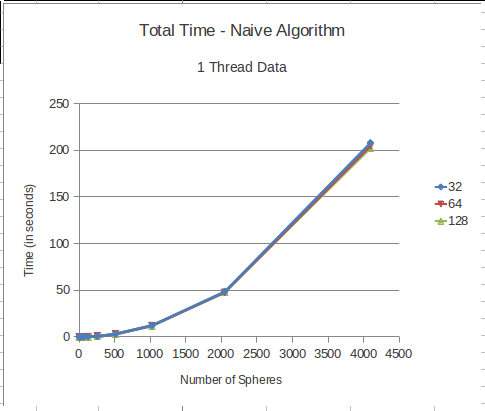
\includegraphics[width=.45\textwidth]{runtime_naive_1thread.png}
	\captionof{figure}{}
	\label{rt_naive1}
\end{figure}
\end{center}

\begin{center}
\begin{figure}
	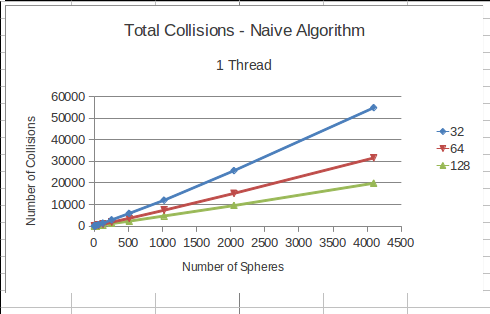
\includegraphics[width=.45\textwidth]{collisions_naive_1thread.png}
	\captionof{figure}{}
	\label{col_naive1}
\end{figure}
\end{center}

For the predictive algorithm, total runtime is not scale-invariant, as predictions rely on calculating physical collisions.  As the volume increases, the likelihood of collision decreases (Figure \ref{rt_predict1}).  Total runtime is showing growth as was true with the naive algorithm, but at a much slower growth rate than the naive algorithm.  This may be a result of extra overhead to perform collision equation calculations in order to reduce the number of unnecessary collision checks.  The number of checks performed per time-step is linear with respect to the number of objects, as opposed to the polynomial growth of the checks performed in the naive solution (Figure \ref{col_predict1}).  Prediction rates were between 0.3\% and 0.7\% correct, which although still low, are enormously more efficient when compared to the naive algorithm (Figure \ref{col_eff}).  These prediction rates are so low because at every time-step, the predictive algorithm still iterates over an array which holds future collision information.  Every array location maps to a sphere, and each location gets 'checked' once per time-step.  So an array location could be 'checked' many times before it actually triggers a collision event.

\begin{center}
\begin{figure}
	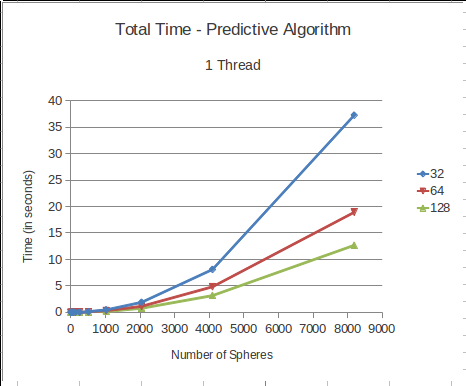
\includegraphics[width=.45\textwidth]{runtime_predictive_1thread.png}
	\captionof{figure}{}
	\label{rt_predict1}
\end{figure}
\end{center}

\begin{center}
\begin{figure}
	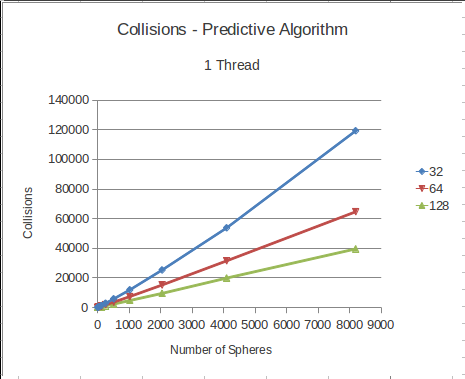
\includegraphics[width=.45\textwidth]{collisions_predictive_1thread.png}
	\captionof{figure}{}
	\label{col_predict1}
\end{figure}
\end{center}

\begin{center}
\begin{figure}
	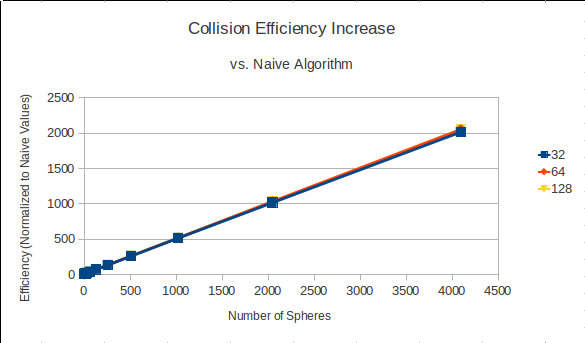
\includegraphics[width=.45\textwidth]{collision_efficiency.png}
	\captionof{figure}{}
	\label{col_eff}
\end{figure}
\end{center}

When subjecting the naive solution to thread improvements, multiple threads offer faster run times as the number of spheres increases (Figure \ref{rt_naive8}).  Total collisions detected are thread-invariant (as they should be), and scale linearly with the number of spheres in the scene (Figure \ref{col_naive8}).  Total checks are also thread-invariant (as they should be), and scale polynomially with the number of spheres in the scene.

\begin{center}
\begin{figure}
	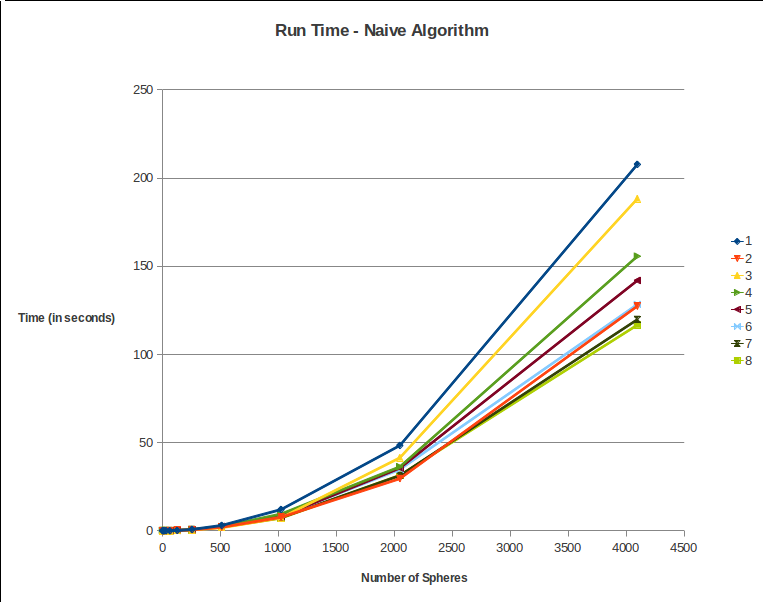
\includegraphics[width=.45\textwidth]{runtime_naive_allthreads.png}
	\captionof{figure}{}
	\label{rt_naive8}
\end{figure}
\end{center}

\begin{center}
\begin{figure}
	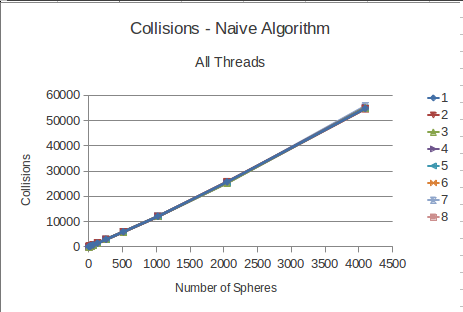
\includegraphics[width=.45\textwidth]{collisions_naive_allthreads.png}
	\captionof{figure}{}
	\label{col_naive8}
\end{figure}
\end{center}

Although single-threaded runs of the predictive algorithm show polynomial growth, it appears that multiple threads of the predictive algorithm begin to exhibit closer to linear growth.  As the number of spheres increases, the benefit of multiple threads increases as well (Figure \ref{rt_predict8}).  Collisions and checks are also thread-invariant (as they should be), and with the predictive algorithm, both scale linearly with the number of spheres in the scene (Figure \ref{col_predict8}).

\begin{center}
\begin{figure}
	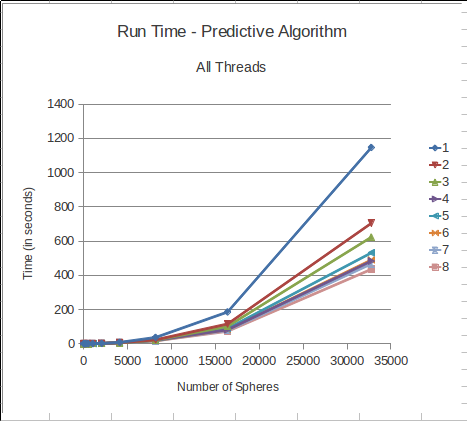
\includegraphics[width=.45\textwidth]{runtime_predictive_allthreads.png}
	\captionof{figure}{}
	\label{rt_predict8}
\end{figure}
\end{center}

\begin{center}
\begin{figure}
	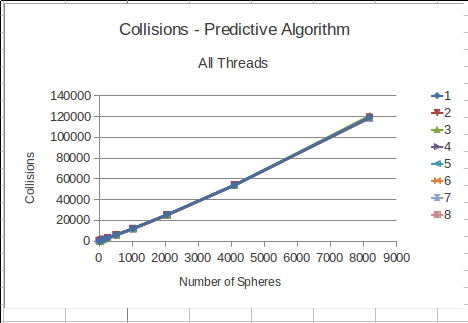
\includegraphics[width=.45\textwidth]{collisions_predictive_allthreads.png}
	\captionof{figure}{}
	\label{col_predict8}
\end{figure}
\end{center}

When comparing the run-times of both algorithms and all thread scenarios, the predictive algorithm appears at this resolution to be linear with respect to the naive algorithm.  However, with the addition of a few extra simulations with even more spheres, we know this is not the case (Figure \ref{rt_predict8}).  The run-times do begin to exhibit a polynomial growth rate, albeit at a much slower growth.  For example, in our data, the predictive algorithm can handle four times as many spheres (shown by the 4096 naive spheres simulation runs just slightly longer than 16384 predictive spheres simulation) to execute in approximately the same runtime as the naive algorithm (Figure \ref{rt_compare}).

\begin{center}
\begin{figure}
	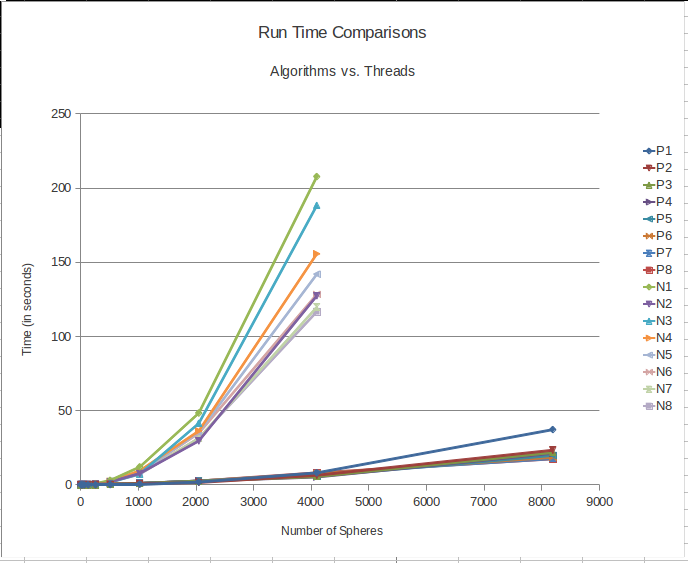
\includegraphics[width=.45\textwidth]{runtime_comparison.png}
	\captionof{figure}{}
	\label{rt_compare}
\end{figure}
\end{center}

With respect to the naive algorithm, the number of checks skyrocket quickly as the number of spheres increases.  In order to more easily visualize the magnitude of this increase, we have shown a log-log plot of the number of spheres for the simulation vs. the number of checks performed by each algorithm.  The plot shows that the number of checks performed in the naive algorithm quickly grows to at least 10 orders of magnitude (base 2) more than the predictive algorithm (Figure \ref{log_checks_compare}).

\begin{center}
\begin{figure}
	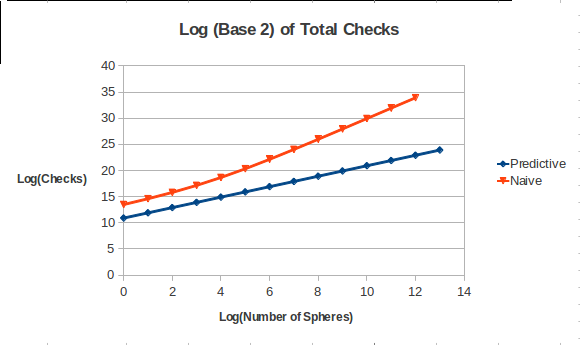
\includegraphics[width=.45\textwidth]{log_total_checks_comparison.png}
	\captionof{figure}{}
	\label{log_checks_compare}
\end{figure}
\end{center}

Next we show that both algorithms eventually gain a benefit from multi-threading, in comparison with their single threaded counterparts (Figures \ref{scalability_naive} and \ref{scalability_predict}).  In addition to the faster run-times of the predictive algorithm, it also scales better than the naive solution as the number of spheres increases.  There is, however, a threshold on the predictive algorithm where there is no threading benefit (in our data, this threshold is between 2048 and 4096 spheres).  This could be caused by some kind of overhead in managing the threads that is a significant portion of the total runtime when there are very few spheres (the predictive algorithm runtime between 2048 and 4096 spheres is 2-8 seconds).  As the number of spheres increases, that overhead appears to become less and less dominant, and the performance improvement can be seen.  At 32768 spheres, the speedup with 8 threads is shown to be 2.6 times faster than the single threaded simulation (Figure \ref{scalability_predict}).

\begin{center}
\begin{figure}
	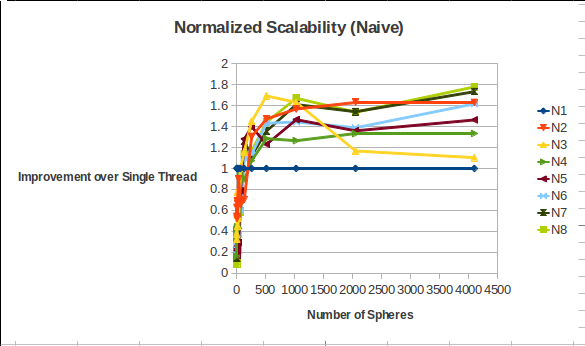
\includegraphics[width=.45\textwidth]{normalized_scalability_naive.png}
	\captionof{figure}{}
	\label{scalability_naive}
\end{figure}
\end{center}

\begin{center}
\begin{figure}
	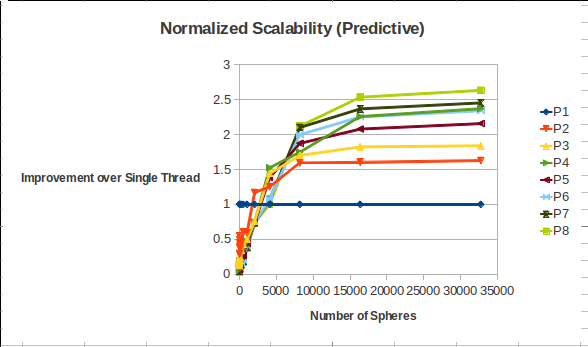
\includegraphics[width=.45\textwidth]{normalized_scalability_predictive.png}
	\captionof{figure}{}
	\label{scalability_predict}
\end{figure}
\end{center}

\section{Conclusion} 

We have presented a novel algorithm to perform discrete event n-body simulations, using predictive event detection instead of polling collision detection.  Our algorithm runs in $O(n)$ time in the average-case for a single time-step.  We have demonstrated that this algorithm has significantly increased single-threaded performance over the naive implementation, and we have presented an implementation that scales well to a multi-core architecture in comparison to the naive algorithm.

\bibliographystyle{IEEEtran}
\bibliography{IEEEabrv,midterm}

\appendix %Steven
\subsection{Prediction Algorithm for Two Spheres}
\label{predict}
This algorithm is relatively simple.  Given two spheres, we can describe their positions, accelerations, and velocities as the equation set.

\begin{eqnarray*}
\vec{p_a}(t)&=&\vec{s_a}+\vec{v_a} t+\vec{a_a} \frac{t ^ 2}{2} \\
\vec{p_b}(t)&=&\vec{s_b}+\vec{v_b} t+\vec{a_b} \frac{t ^ 2}{2} \\
\end{eqnarray*}

Then, we find when/if the distance between the two spheres is equal to the sum of their radii.  

\begin{eqnarray*}
|| \vec{p_b}(t)-\vec{p_a}(t) ||&=&r_a+r_b \\
|| \vec{p_b}(t)-\vec{p_a}(t) || ^ 2&=&(r_a+r_b) ^ 2 \\
\end{eqnarray*}

This can be expanded as a quartic polynomial in terms of the difference between their two positions, eg, p is the view of a from b's frame of reference.
  
\begin{equation}
\vec{p}(t)=\vec{p_a}(t)-\vec{p_b}=\vec{s}+\vec{v} t+\vec{a} \frac{t ^ 2}{2}
\end{equation}

then, the expanded squared norm of p is a quartic polynomial

\begin{eqnarray*}
	|| \vec{p}(t) || ^ 2 &=&\vec{s} \cdot \vec{s} \\
	&+&2 \vec{s} \cdot \vec{v} t \\
	&+& (\vec{s} \cdot \vec{a} \\ 
	&+&  \vec{v} \cdot \vec{v}) t ^ 2 \\
	&+& \vec{a} \cdot \vec{v} t ^ 3 \\
	&+& \frac{\vec{a} \cdot \vec{a}}{4} t ^ 4 \\
	&=& (r_a+r_b) ^ 2 \\
\end{eqnarray*}

When acceleration is constant, then the difference of the two acceleration reference frames $a$ is 0, and the above reduces to a quadratic that can be solved using the quadratic formula.
When acceleration is not constant, then the above reduces to a quartic equation that can be solved for $t$ as well.   In either case, if $t$ any positive real solutions, then the smallest of these 
is taken as the predicted collision time.  Otherwise, no collision is predicted. 




\begin{comment}
\begin{thebibliography}{99}
\bibitem{journal-1} Akbar M.M., Manning E.G., Shoja G.C., Khan S., Heuristic Solutions for the Multiple-Choice Multi-dimension Knapsack Problem, LECT NOTES COMPUT SC, 2001, 2074, 659-668
\bibitem{journal-2} Kemerer C.F., Slaughter S., An empirical approach to studying software evolution, IEEE T SOFTWARE ENG, 2002, 25, 493-509 
\bibitem{journal-3} Moshkov M.Ju., The depth of decision trees for binary problems, Vestnik Moskovskogo Universiteta, Matematika, Mekhanika, 2007, 62(3), 25-29 (in Russian)
\bibitem{journal-4} Wieczorek W., An algorithm for the decomposition of finite languages, Logic Journal of the IGPL, doi:10.1093/jigpal/jzp032, 2009, 12
\bibitem{journal-5} Tekli J., Damiani E., Chbeir R., Gianini G., SOAP Processing Performance and Enhacement, IEEE TSC, (in press)
\bibitem{book-1} Agrawal D.P., Zeng Q.A., Introduction to Wireless and Mobile Systems, Third Edition, Cengage Learning, Stamford, CT, USA, 2011
\bibitem{book-2} Astrom K.J., Wittenmark B., Adaptive Control, 2nd Edition, Addison-Wesley Longman Publishing Co., Boston, MA, USA, 1994
\bibitem{chapter} Dorigo M., St{\"u}tzle T., Ant Colony Optimization: Overview and Recent Advances, In: Gendreau M., Potvin J.-Y. (Eds.), Handbook of Metaheuristics, International Series in Operations Research and Management Science vol. 146, Springer US, New York, 2010
\bibitem{arxiv-1} Majewski, M., Malarz, K., arXiv:cond-mat/0609635v2
\bibitem{proceedings} Dougherty B., White J., Thompson C., Schmidt D., Automating Hardware and Software Evolution Analysis, In: Bapty T. (Ed.), International Conference and Workshop on the Engineering of Computer Based Systems (ECBS) (November 2009, San Francisco, USA), IEEE Computer Society, 2009, 265-274
\bibitem{thesis} Wang Y., Application-Specific Quality of Service Constraint Design in Wireless Sensor Networks, PhD Thesis, University of Cincinnati, Cincinnati, June 14, 2008 
\bibitem{newspaper-1} Sherwin, A., The Times, 13 Jul. 2007, 1
\bibitem{newspaper-2} Dzierzanowski, M., Wprost, 8 Jul. 2007, 18 (in Polish)
\bibitem{patent} Philip Morris Inc., European patent application 0021165 A1, 1981.01.07
\bibitem{standard-1} ISO 2108:1992, Information and documentation --- International standard book numbering (ISBN)
\bibitem{standard-2} ISO/TR 9544:1988, Information processing --- Computer-assisted publishing --- Vocabulary
\end{thebibliography}
\end{comment}

\end{document}
